% --------------------------------------
% Document Class
% --------------------------------------
\documentclass[a4paper,11pt]{article}
% --------------------------------------



% --------------------------------------
% Use Package
% --------------------------------------


\usepackage[francais]{babel}
%\usepackage{ucs}
\usepackage[utf8]{inputenc}
\usepackage[T1]{fontenc}

\usepackage{makeidx}
\usepackage{color}
\usepackage{graphicx}
\usepackage{float}
\usepackage[hidelinks]{hyperref} 
\usepackage{geometry}
%\usepackage{lastpage}
%\usepackage{marginnote}
\usepackage{fancyhdr}
%\usepackage{titlesec}
%\usepackage{framed}
\usepackage{amsmath}
\usepackage{empheq}
\usepackage{array}
\usepackage{multicol}
\usepackage{csquotes}
%\usepackage{adjustbox}

% insert code
\usepackage{listings}

% define our color
\usepackage{xcolor}

% code color
\definecolor{ligthyellow}{RGB}{250,247,220}
\definecolor{darkblue}{RGB}{5,10,85}
\definecolor{ligthblue}{RGB}{1,147,128}
\definecolor{darkgreen}{RGB}{8,120,51}
\definecolor{darkred}{RGB}{160,0,0}

% other color
\definecolor{ivi}{RGB}{141,107,185}


\lstset{
    language=Scilab,
    captionpos=b,
    extendedchars=true,
    frame=lines,
    numbers=left,
    numberstyle=\tiny,
    numbersep=5pt,
    keepspaces=true,
    breaklines=true,
    showspaces=false,
    showstringspaces=false,
    breakatwhitespace=false,
    stepnumber=1,
    showtabs=false,
    tabsize=3,
    basicstyle=\small\ttfamily,
    backgroundcolor=\color{ligthyellow},
    keywordstyle=\color{ligthblue},
    morekeywords={include, printf, uchar},
    identifierstyle=\color{darkblue},
    commentstyle=\color{darkgreen},
    stringstyle=\color{darkred},
}


% --------------------------------------



% --------------------------------------
% Page setting
% --------------------------------------
%\pagestyle{empty}
\setlength{\headheight}{15pt}

\setcounter{secnumdepth}{3}
\setcounter{tocdepth}{2}

\makeatletter
\@addtoreset{chapter}{part}
\makeatother 

\hypersetup{         % parametrage des hyperliens
  colorlinks=true,      % colorise les liens
  breaklinks=true,      % permet les retours à la ligne pour les liens trop longs
  urlcolor= blue,       % couleur des hyperliens
  linkcolor= black,     % couleur des liens internes aux documents (index, figures, tableaux, equations,...)
  citecolor= green      % couleur des liens vers les references bibliographiques
}

% --------------------------------------

% --------------------------------------
% Information
% --------------------------------------
\title{Compte-rendu TP6 TI : Classification automatique de textures cycliques par analyse du plan de Fourier}
\author{Elliot VANEGUE et Gaëtan DEFLANDRE}
% --------------------------------------

\definecolor{myColor}{rgb}{0.5, 0.1, 0.75}

% --------------------------------------
% Begin content
% --------------------------------------
\begin{document}

% Set language to english
  \selectlanguage{francais}

  % Start the page counting
  \pagenumbering{arabic}

  \maketitle
  
  \mbox{}
  \newpage
  \clearpage
  
  \section*{Introduction}
  L'objectif de ce TP était de découvrir comment nous pouvons représenter les fréquences à l'intérieur 
  d'une image. Nous avons étudié la transformée de Fourier afin de comprendre son fonctionnement et 
  d'extraire différentes caractéristiques d'une image.
  
  \section{Fréquence spatiale}
  Lors de ce TP, nous avons travaillé avec des images composées de raillure afin de pouvoir
  facilement travailler sur les fréquences d'une image.\\
  
  Dans un premier temps nous avons calculé la période des images, c'est à dire le nombre de fois 
  qu'un motif se répète. Nous avons trouvé, pour les image \enquote{*\_a.jpg}, une période de 5 pixels pour toute les images. En effet,
  ces images change de dimension, mais la période du motif ne change pas. Cela nous donne donc
  une fréquence spatiale de $\frac{1}{5}$.
  
  \section{Raie maximale d'une image}
  
  Nous avons abord changé le plan de cette image pour que les descripteurs soit compris entre -0,5
  et 0,5 afin de se border aux fréquences maximales d'une image. Pour cela, nous avons appliqué la 
  macro suivante sur chaque point du graphique.
  
  \begin{lstlisting}[caption=Fonctions de passage aux coordonnées dans le plan de Fourier]
  function fourierXCoordinate(imgXCoordinate, width) {
    return (imgXCoordinate/width) - 0.5;
  }

  function fourierYCoordinate(imgYCoordinate, height) {
    return ((imgYCoordinate/height) - 0.5) * -1;
  }
  \end{lstlisting}
  
  Dans ce calcule, nous divisons par width ou height afin de passer à un repère (0,1), puis nous effectuons une 
  soustraction dans le but de se ramener à un repère (-0.5,0.5). Ce changement de repère nous permet de placer
  les basses fréquences au centre du graphique.
  
  La raie maximale de l'image se trouve au centre du plan de Fourier (coordonnées [0;0]). Elle représente la 
  composante continue à la fréquence nulle qui est la moyenne de l'image. Cette composante est utilisée lors des
  calculs de la transformée. Elle n'est pas significative des fréquences de l'image.
  
  \begin{figure}[H]
  \center
   \includegraphics[width=5cm]{FFT256a.png}
   \caption{Représentation déscripteurs de Fourier avec la raie maximale au centre}
  \end{figure}

  
  \section{Second valeur maximale d'une image}
  
  Nous avons ensuite recherché la second valeur maximale de l'image grâce la macro suivante :
  \begin{lstlisting}[caption=Fonctions de passage aux coordonnées dans le plan de Fourier]
  for (j=0; j<H; j++)
    {
        for (i=0; i<W; i++) 
        {
            p = getPixel(i,j);
            if ( max_1 < p)
            {
                max_2 = max_1;
                i_max_2 = i_max_1;
                j_max_2 = j_max_1;
                max_1 =p;
                i_max_1 = i;
                j_max_1 = j;
            } 
        }
    }
  \end{lstlisting}
  
  %TODO ajout -> précise la fréquence
  Cette seconde valeur va nous fournir deux informations :
  \begin{itemize}
   \item La fréquence du motif
   \item l'orientation des motifs de l'image : la droite passant
  par les deux valeurs maximales est perpendiculaire au motif. Ce qui signifie que si la droite est horizontal
  alors les motifs de l'image se répète verticalement.
  \end{itemize}

  Cette second valeur va nous permettre de déterminer l'orientation des motifs de l'image. La droite passant
  par les deux valeurs maximales est perpendiculaire au motif. Ce qui signifie que si la droite est horizontal
  alors les motifs de l'image se répète verticalement.
  
  \begin{figure}[H]
  \center
   \includegraphics[width=5cm]{FFT256a.png}
   
\includegraphics[width=5cm]{256_a.jpg}
   \caption{Image avec une répétition de motif et son graphique de descripteurs de Fourier}
  \end{figure}
  
  Nous avons remarqué que si des images ont la même fréquence, mais avec une orientation de répétition de motif
  différente alors ces images auront les mêmes maximales.\\
  
  Nous avons également constaté que la transformée de l'image du damier de période deux pixels donne une transformée 
  qui n'est pas totalement visible sur l'image retournée par Imagej. En effet, on retrouve un point dans les hautes 
  fréquences, $f=\frac{1}{2}$, cependant on devrait retrouver trois autres points dans les coins de l'image. Cela est lié à la 
  représentation de point au sens mathématique par des pixels. Les quatre points sont bien calculés, mais trois des pixels 
  se retrouvent à l'extérieur du cadre.\\
  
  \begin{tabular}{|c|c|c|}
  \hline
   image & graphique des descripteurs de Fourier & seconde maximale \\
  \hline
  256\_a & \includegraphics[width=5cm]{FFT256a.png} & 0,1992\\
  \hline
  256\_b & 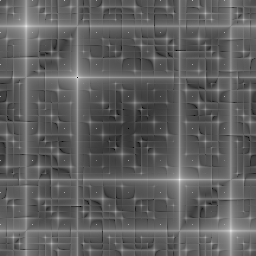
\includegraphics[width=5cm]{FFT256b.jpg} & 0,1992\\
  \hline
  256\_d & \includegraphics[width=5cm]{FFT256d.png} & 0,1016\\
  \hline
  \shortstack{
\includegraphics[width=3cm]{../gaetan/images/damier32x32.png} \\ damier 1 pixel} & 
\includegraphics[width=3cm]{FFTD32.png} & 0,1016\\
  \hline
  \end{tabular}
  
  \section*{Conclusion}
  
  Lors de ce TP, nous avons constaté qu'il était possible de représenter les fréquences d'une image grâce à la 
  transformation de Fourier. Cette transformée permet de retrouver les directions et la période de motif au sein 
  d'une image. La transformée de Fourier pourrait être utilisée pour détecter des textures qui se répètent dans une
  image. Il est également possible de retrouver une image à partir de la transformée de Fourier.
  
  \newpage
  \section*{Annexe}
  
  \begin{lstlisting}[caption=Macro complète du TP]
macro "direction FFT"
{
  // ouverture d'une image si necessaire - sinon la macro analyse l'image courante
  //open ("/home/bmathon/Enseignement/TI/tp6_TF/images/256_a.jpg");

  // recuperation de l'identifiant de l'image
  image = getImageID();

  // application de la TDF (FFT : Fast Fourier Transform)
  run("FFT");

  // recuperation de l'ID du module de la FFT
  fourier = getImageID();

  // recuperation de la taille W x H du module de la FFT
  W = getWidth();
  H = getHeight();

  // recherche du max
  max_1 = 0; 
  i_max_1 = 0;
  j_max_1 = 0;

  max_2 = 0; 
  i_max_2 = 0;
  j_max_2 = 0;

  for (j=0; j<H; j++)
  {
    for (i=0; i<W; i++) 
    {
      p = getPixel(i,j);
      if ( max_1 < p)
      {
        max_2 = max_1;
        i_max_2 = i_max_1;
        j_max_2 = j_max_1;

        max_1 = p;
        i_max_1 = i;
        j_max_1 = j;
      } 
    }
  }

  // mise a zero de la valeur max

  setPixel (i_max_1,j_max_1,0);

  print("Max 1: " + getFourierCoordinateAsString(i_max_1, j_max_1, W, H));
  print("Max 2: " + getFourierCoordinateAsString(i_max_2, j_max_2, W, H));

  if(fourierXCoordinate(i_max_2,W)==0){
    print("Horizontal"); 
  } else if(fourierYCoordinate(j_max_2,H)==0){
    print("Vertical");
  } else {
    print("Diagonal");
  }

}

function fourierXCoordinate(imgXCoordinate, width) {
  return (imgXCoordinate/width) - 0.5;
}

function fourierYCoordinate(imgYCoordinate, height) {
  return ((imgYCoordinate/height) - 0.5) * -1;
}

function getFourierCoordinateAsString(imgXCoordinate, imgYCoordinate, width, height) {
  fourierX = fourierXCoordinate(imgXCoordinate, width);
  fourierY = fourierYCoordinate(imgYCoordinate, height);
  text = "[x:" + fourierX + ", y:" + fourierY + "]";
  return text;
}
  \end{lstlisting}
  
\end{document}  